\documentclass[aspectratio=169]{beamer}

\usetheme{Madrid}
\usecolortheme{default}
\setbeamertemplate{navigation symbols}{}
\setbeamertemplate{footline}[frame number]

\usepackage[utf8]{inputenc}
\usepackage[T1]{fontenc}
\usepackage{lmodern}
\usepackage{booktabs}
\usepackage{array}
\usepackage{ragged2e}
\usepackage{tikz}
\usetikzlibrary{positioning}

\definecolor{Primary}{RGB}{17,47,65}
\definecolor{Accent}{RGB}{183,137,61}
\definecolor{Soft}{RGB}{242,245,247}
\definecolor{Good}{RGB}{35,110,75}
\definecolor{Warn}{RGB}{170,92,42}

\setbeamercolor{palette primary}{bg=Primary, fg=white}
\setbeamercolor{palette secondary}{bg=Primary, fg=white}
\setbeamercolor{palette tertiary}{bg=Primary, fg=white}
\setbeamercolor{palette quaternary}{bg=Primary, fg=white}
\setbeamercolor{structure}{fg=Primary}
\setbeamercolor{title}{fg=Primary}
\setbeamercolor{frametitle}{fg=Primary, bg=Soft}
\setbeamercolor{block title}{bg=Primary, fg=white}
\setbeamercolor{block body}{bg=Soft, fg=black}

\title{Legal Query System}
\subtitle{Project Progress Presentation}
\author{Project Team}
% \institute{Current Implementation Review}
% \date{April 10, 2026}


\begin{document}

\begin{frame}[plain]
  \begin{center}
    \vspace*{0.5cm}
    % Title and Subtitle
    {\Large \textbf{\textcolor{Primary}{Legal Query System with Exact Law References}}}\\[0.5em]
    {\Large \textbf{\textcolor{Accent}{Project Progress Presentation}}}\\[1em]

    % Guide
    {\small Guided by: \textbf{\textcolor{Good}{Dr. Kaushledra Kumar Singh}}} \\[0.2cm]
    {\small and \textbf{\textcolor{Good}{Anand Kumar Ohm}}}
  \end{center}

  \vfill

  % Problem Statement Block
  % \begin{block}{Problem Statement}
  %   \justifying\small
  %   Legal information is available in official PDFs, but finding the right section quickly is difficult for students and non-expert users. Our project aims to reduce that effort by combining a searchable legal corpus with a conversational interface that returns answers along with source-backed citations.
  % \end{block}

  \vfill

  % Project Members Table
  \begin{center}
    \small
    \renewcommand{\arraystretch}{1.2}
    \begin{tabular}{@{}ll@{}}
      \toprule
      \textbf{Project Members} & \textbf{Roll Number} \\
      \midrule
      Sujal Kumar (Group Leader) & 2023UGCS076 \\
      Tanishq Gupta & 2023UGCS074 \\
      Saurabh Kumar & 2023UGCS040 \\
      Sujal Bhatu & 2023UGCS119 \\
      \bottomrule
    \end{tabular}
  \end{center}

  \vfill

  % Footer info
%   \begin{center}
%     \scriptsize
%     Current Implementation Review \quad $\bullet$ \quad April 10, 2026
%   \end{center}
\end{frame}

\begin{frame}{Problem We Are Solving}
  \justifying
  % Legal information is available in official PDFs, but finding the right section quickly is difficult for students and non-expert users. Our project aims to reduce that effort by combining a searchable legal corpus with a conversational interface that returns answers along with source-backed citations.

  Finding the right sections in official PDFs has been very difficult task for naive users. The objective is to develop an AI-powered legal query assistant that answers situation-specific
legal questions by retrieving and citing exact law sections, act numbers, sub-clauses, and relevant case precedents from a curated statutory corpus.

  \vspace{0.5em}
  \begin{block}{Core Idea}
    Build a legal assistant which can accept natural language questions, retrieve relevant statutory text, and present a readable answer with supporting clauses.
  \end{block}
\end{frame}

\begin{frame}{Project Objectives}
  \begin{itemize}
    \item Develop a simple web interface to provide an answer to legal questions
    \item Users can authenticate and have a "persistent chat session"
    \item Question and answer will use an information retrieval pipeline over Indian Law Database
    % \item Return answers with cited sources instead of plain uncited text.
    \item Answers returned are from cited sources instead of plain uncited text.
    \item Metadata is used to maintain source traceablility for official government documents.
   % \item Maintain source traceability using metadata from official government documents.
  \end{itemize}
\end{frame}

\begin{frame}{Current Progress Snapshot}
  \begin{table}
    \centering
    \renewcommand{\arraystretch}{1.35}
    \begin{tabular}{>{\RaggedRight\arraybackslash}p{0.36\linewidth} >{\RaggedRight\arraybackslash}p{0.52\linewidth}}
      \toprule
      \textbf{Module} & \textbf{Current Status} \\
      \midrule
      Frontend UI & Implemented with React, Vite, route-based pages, dashboard, and chat screen \\
      Authentication & Signup, login, JWT-based session handling, protected routes implemented \\
      Backend API & Express server with auth routes and chat session management implemented \\
      Database Layer & MongoDB models for users and chat sessions implemented \\
      RAG API & Flask service created for query handling and ingestion trigger \\
      Retrieval Pipeline & Embedding, Chroma-based search, prompt assembly, and source formatting implemented \\
      Legal Corpus & 18 legal PDF sources listed in metadata manifest; current workspace has one extracted and chunked sample document ready for retrieval validation \\
      \bottomrule
    \end{tabular}
  \end{table}
\end{frame}

\begin{frame}{System Architecture}
  \centering
  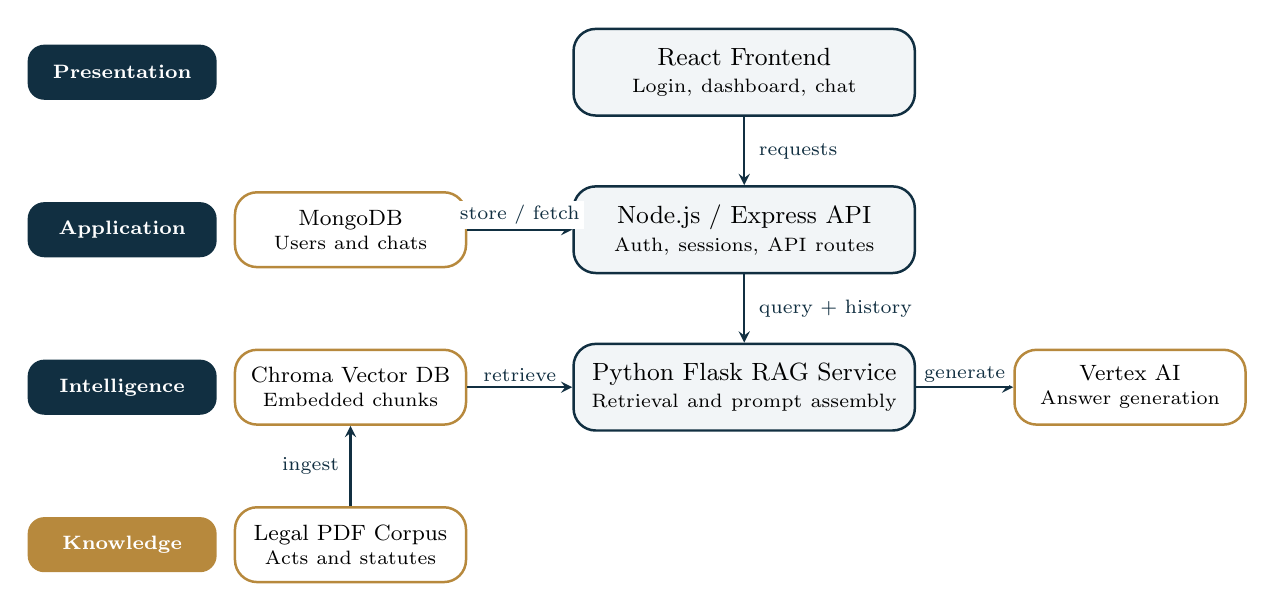
\begin{tikzpicture}[
    x=1cm,
    y=1cm,
    every node/.style={align=center},
    layerlabel/.style={
      draw=none,
      fill=Primary,
      text=white,
      rounded corners=6pt,
      minimum width=2.4cm,
      minimum height=0.7cm,
      font=\scriptsize\bfseries
    },
    layerbox/.style={
      draw=Primary,
      rounded corners=8pt,
      fill=Soft,
      text width=4.1cm,
      minimum height=1.0cm,
      line width=0.9pt,
      font=\small
    },
    datastore/.style={
      draw=Accent,
      rounded corners=8pt,
      fill=white,
      text width=2.7cm,
      minimum height=0.95cm,
      line width=0.9pt,
      font=\footnotesize
    },
    flow/.style={->, thick, color=Primary, >=stealth},
    note/.style={font=\scriptsize, text=Primary, fill=white, inner sep=1.5pt}
  ]

    % Left hierarchy labels
    \node[layerlabel] at (-6.8,0) {Presentation};
    \node[layerlabel] at (-6.8,-2.0) {Application};
    \node[layerlabel] at (-6.8,-4.0) {Intelligence};
    \node[layerlabel, fill=Accent] at (-6.8,-6.0) {Knowledge};

    % Main hierarchy backbone
    \node[layerbox, minimum height=1.1cm] (ui) at (1.1,0) {React Frontend\\[-0.1em]\scriptsize Login, dashboard, chat};
    \node[layerbox, minimum height=1.1cm] (api) at (1.1,-2.0) {Node.js / Express API\\[-0.1em]\scriptsize Auth, sessions, API routes};
    \node[layerbox, minimum height=1.1cm] (rag) at (1.1,-4.0) {Python Flask RAG Service\\[-0.1em]\scriptsize Retrieval and prompt assembly};

    % Support systems placed in separate columns
    \node[datastore] (mongo) at (-3.9,-2.0) {MongoDB\\[-0.1em]\scriptsize Users and chats};
    \node[datastore] (vector) at (-3.9,-4.0) {Chroma Vector DB\\[-0.1em]\scriptsize Embedded chunks};
    \node[datastore] (pdf) at (-3.9,-6.0) {Legal PDF Corpus\\[-0.1em]\scriptsize Acts and statutes};
    \node[datastore] (llm) at (6.0,-4.0) {Vertex AI\\[-0.1em]\scriptsize Answer generation};

    % Main flow arrows
    \draw[flow] (ui) -- (api) node[midway, right=0.12cm, note] {requests};
    \draw[flow] (api) -- (rag) node[midway, right=0.12cm, note] {query + history};

    % Side relationships
    \draw[flow] (mongo.east) -- (api.west) node[midway, above, note] {store / fetch};
    \draw[flow] (vector.east) -- (rag.west) node[midway, above, note] {retrieve};
    \draw[flow] (rag.east) -- (llm.west) node[midway, above, note] {generate};
    \draw[flow] (pdf.north) -- (vector.south) node[midway, left=0.08cm, note] {ingest};
  \end{tikzpicture}
\end{frame}

\begin{frame}{How the System Works}
  \begin{enumerate}
    \item User signs up or logs in through the frontend.
    \item Frontend sends the credentials to the Express backend.
    \item Backend verifies the user data and returns a JWT token.
    \item User opens a chat session and enters a legal query.
    \item Backend forwards the query and recent chat history to the Python RAG API.
    \item RAG pipeline retrieves relevant legal chunks from the vector database.
    \item Retrieved context is sent to the LLM to generate a readable answer.
    \item Final answer and citations are returned, displayed, and stored in the chat session.
  \end{enumerate}
\end{frame}

\begin{frame}{Frontend and Backend Work Completed}
  \begin{columns}[T]
    \column{0.49\linewidth}
    \begin{block}{Frontend}
      \begin{itemize}
        \item Route-based app structure
        \item Login and signup pages
        \item Protected dashboard
        \item Chat interface with message history
        \item Citation cards for legal sources
        \item Session solved/active workflow
      \end{itemize}
    \end{block}

    \column{0.49\linewidth}
    \begin{block}{Backend}
      \begin{itemize}
        \item Express API setup
        \item JWT authentication middleware
        \item MongoDB models for users and chat sessions
        \item Session creation, listing, deletion, and update routes
        \item Integration with Python RAG service
      \end{itemize}
    \end{block}
  \end{columns}
\end{frame}

\begin{frame}{RAG Pipeline Progress}
  \begin{itemize}
    \item PDF ingestion pipeline extracts text and creates legal chunks.
    \item Metadata manifest stores source title, year, authority, URLs, and file hash.
    \item SentenceTransformer embeddings are used for semantic search.
    \item ChromaDB stores chunk embeddings for retrieval.
    \item Prompt design is focused on simple answers with legal citations and disclaimer.
    \item The pipeline supports either Vertex AI or an OpenAI-compatible provider.
  \end{itemize}

  \vspace{0.4em}
  \begin{block}{Important Note on Current State}
    The source library has been assembled for 18 documents, while the visible chunked data in the current workspace shows one processed sample document. This is enough to validate the flow, but full-corpus indexing is still part of the next execution step.
  \end{block}
\end{frame}

\begin{frame}{Current Progress}
  \begin{itemize}
    \item An end-to-end application path is now available
    \item Logic for retrieval and core backend  are working fine
    \item metadata for the source improves traceability and system becomes more presentation-worthy and audit-friendly.
    \item The present build : user management, query flow, storage, retrieval, and answer rendering are all connected.
  \end{itemize}
\end{frame}

\begin{frame}{Current Limitations}
  \begin{itemize}
    \item Full ingestion across all collected legal PDFs has not yet been materialized in the current workspace output.
    \item Furthermore, the accuracy still depends upon the quality of the chunks, retrieval quality, and prompt behavior.
    \item This system is designed to assist users in finding legal information and NOT to provide them with formal legal advice.
    \item More evaluation is needed for edge cases, ambiguous queries, and multi-act comparisons.
    % \item Production-grade concerns such as role-based access, monitoring, and broader testing are future work.
  \end{itemize}
\end{frame}

\begin{frame}{Next Milestones}
  \begin{itemize}
    \item Rebuild the vector store for the full legal corpus.
    \item Expand the number of acts being tested and more diverse legal queries.
    \item Improve answer formatting and citation confidence.
    \item Add stronger evaluation for accuracy and retrieval quality.
    \item Enhance dashboard analytics and query management features.
    % \item Prepare the system for a cleaner demo and future deployment.
  \end{itemize}
\end{frame}

\begin{frame}{Conclusion}
  \justifying
  We have made a working legal inquiry platform using modern web technologies for retrieval-augmented generation. The front-end, back-end, authentication methods, session storage and RAG workflow have been successfully integrated.
  \vspace{0.8em}
  \centering
  % {\large \textbf{Thank You}}

  \vspace{0.3em}
  % Questions and suggestions are welcome.
\end{frame}

\end{document}
